\documentclass[conference]{IEEEtran}
\IEEEoverridecommandlockouts
% The preceding line is only needed to identify funding in the first footnote. If that is unneeded, please comment it out.
\usepackage{cite}
\usepackage{amsmath,amssymb,amsfonts}
\usepackage{algorithmic}
\usepackage{url}
\usepackage{graphicx}
\usepackage{textcomp}
\usepackage{xcolor}
\usepackage{tikz}
\def\BibTeX{{\rm B\kern-.05em{\sc i\kern-.025em b}\kern-.08em
    T\kern-.1667em\lower.7ex\hbox{E}\kern-.125emX}}
\begin{document}
\title{Formally Verifying Voter Security Properties in DAO Smart Contracts}

\author{
    \makebox[\textwidth][c]{%
        \begin{minipage}{0.45\textwidth}
            \centering
            \textbf{Anish Toomu} \\
            \textit{Department of Computer Science} \\
            \textit{University of North Carolina at Chapel Hill} \\
            Chapel Hill, North Carolina, USA
        \end{minipage}
        \hfill
        \begin{minipage}{0.45\textwidth}
            \centering
            \textbf{Aidan Maguire} \\
            \textit{Department of Computer Science} \\
            \textit{University of North Carolina at Chapel Hill} \\
            Chapel Hill, North Carolina, USA
        \end{minipage}
    }\\[1.5em]

    \makebox[\textwidth][c]{%
        \begin{minipage}{0.6\textwidth}
            \centering
            \textbf{Jeffrey Zhang} \\
            \textit{Department of Computer Science} \\
            \textit{University of North Carolina at Chapel Hill} \\
            Chapel Hill, North Carolina, USA
        \end{minipage}
    }
}

\maketitle






\section{Introduction}
This project aims to make use of two existing security tools to define and verify security properties for voting methods across a suite of Ethereum blockchain programs. Many Ethereum blockchain programs take the form of a DAO, or Decentralized Autonomous Organization, wherein users holding tokens that verify them as members of the organization can spend those tokens to vote on decision-making for the DAO as a whole. There are several types of vulnerabilities that have been identified in these types of contracts, but for this paper we will be looking at vulnerabilities surrounding the vote system that allow attackers to exploit the democratic principles behind DAOs.

Our proposal intends to formally verify a suite of the most used DAO contracts to confirm that they are secure. We will require the use of Scribble, a specification language that allows us to define security properties for DAO contracts as annotations within the contracts themselves. We will then use Mythril, a security-analysis tool, to verify each of our newly defined security properties for our suite of popular contracts. If successful, we will increase the confidence in these widely-used contracts. Possible challenges include the properties not being entirely specifiable in Scribble's specification language, and some contracts being too complex to analyze with Mythril due to state explosion.

\section{State of the Art}

DAOs are a type of smart contract that define the rules and structure of a organization. In more general terms, DAOs represent decentralized communities that can allocate resources without centralized leadership. While there exist tools for various methods of verifying and bug-finding in smart contracts including static analysis[1], model checking[2], and symbolic execution[3], they haven’t been narrowed down to focus on DAOs, and the specific exploits that come with their voting systems, a key, shared property across DAOs and a critical part of their operations. We have chosen to use an existing symbolic execution-based tool, Mythril[4], along with Scribble[5], a specification language for properties in this work. 


\section{Background}
To understand our proposed enhancements to Mythril, we must first grasp the fundamental concepts of the blockchain, the Ethereum blockchain and its innovative smart contracts, and finally DAOs, a subset of smart contracts with common functionalities.

\subsection{Blockchain}
A blockchain serves as a ledger of transactions that is transparent, decentralized, and secure. Each block in the chain contains information about transactions allowing anyone to inspect them at any time. Additionally, each block contains a cryptographic hash of the previous block in the chain. This chain means that in the event of a block being tampered with by an attacker, all of the altered blocks' successors would also be changed. The consensus needed to accept a chain also provides further security. If the majority of the computational power on the network is controlled by honest parties then the honest chain will be accepted. An attacker seeking to change a block would need to alter the block, redo all the proof-of-work computation for it and its successor blocks, and then catch up to the honest chain to be accepted. This proves to be computationally infeasible[6].

\subsection{Ethereum and Smart Contracts}
Ethereum, as proposed by Vitalik Buterin in 2014, seeks to provide an alternative to Bitcoin with a focus on the development of decentralized applications. This is achieved through a blockchain that contains a built-in Turing-complete language[7]. This language allows users to write smart contracts that are stored on the blockchain. Smart contracts are a type of account, they have a balance and can be interacted with through transactions. They differ from users’ externally owned accounts in their method of control. Where externally owned accounts are controlled by user decisions, smart contracts are programs that run on the blockchain according to their code. Users or other smart contracts interact with smart contracts by sending a transaction that executes the functions defined by the contract’s code. Smart contracts automatically execute when their conditions are met, are universally visible, and are unable to be changed once uploaded[8]. In this way smart contracts provide a trustworthy, automated way to enforce agreements, reducing the need for third-party enforcement, minimizing exceptions, and lowering the risk of fraud[9].

\subsection{Decentralized Autonomous Organizations}
Decentralized Autonomous Organizations (DAOs) use the blockchain and smart contracts as a way to govern and operate an organization without a central authority. DAOs allow participants to vote on proposed policy changes, actions taken by the organization, and any number of other decisions. These rules are automatically enforced by smart contracts. The first notable DAO, “The DAO” was formed on the Ethereum blockchain in 2016 as a venture capital fund. Users could exchange ether for tokens that gave holders voting power in The DAO proportional to the amount of tokens owned[10]. The organization managed to crowdfund \$168M worth of ether representing one of the largest projects on the Ethereum blockchain. The project is now synonymous with a programming vulnerability in the organization's smart contract that allowed an attacker to siphon off \$50M from The DAO’s[11] gathered funds. This resulted in the controversial hard fork of the Ethereum blockchain and the shuttering of the organization. This example highlights the critical nature of DAO smart contract security as they manage large amounts of currency and interact with a large number of users. Today, a great variety of DAOs exist on Ethereum ranging from communities of creators to venture capital groups[12].

\section{Threat Model}
DAO contract voting vulnerabilities refers to a class of vulnerabilities where an attacker exploits the contract voting mechanism to vote twice with the same tokens, remove other people's votes, vote on a proposal and immediately put it into effect without giving other token holders a chance to vote themselves, or other similar exploits that undermine the decentralized democratic goals of DAO contracts. In our analysis, we assume that attackers have complete visibility of the contract code, and the ability to deploy their own contracts to the blockchain that interface with DAO contracts[13]; however, we are assuming that attackers cannot launch larger Ethereum network attacks such as network congestion or miner manipulation that would require greater coordination and resources. We consider nonvoting-related attacks such as integer overflow, reentrancy, and gas DoS attacks as out of scope for this paper. 

\section{Design}

\subsection{A Formal Model of DAO Smart Contracts}
There is not a prescriptive structure that smart contracts must conform to in order to be considered DAOs, but there are some functionalities that are common to all implementations. All DAOs have a voting function in their contract that allows members to vote on proposals made by other members. We represent the general form of this voting function as a finite state machine that DAO members can interact with. We define the FSM as follows:
\begin{center}
$M = (Q, \Sigma, \delta, q_0, F)$
\end{center}

With $Q$ being the set of contract states, $\Sigma$ being the set of events, $\delta$ being the transition function mapping $Q\times\Sigma$, $q_0$ being the initial state, and $F$ being the set of terminal states. 
We define the set $Q$ as follows:
\begin{center}
\begin{tabular}{|c|c|}
\hline
State & Description\\
\hline
$q_0$ & Initial state. Contract is inert.\\
\hline
A & Vote request initiated. Voter identity set\\
\hline
B & Vote request validated\\
\hline
Y & Vote total updated in favor. Terminate interaction \\
\hline
N & Vote total updated against. Terminate interaction\\
\hline
R & Vote canceled. Terminate interaction\\
\hline
\end{tabular}
\end{center}

And define the set $Sigma$ as follows:
\begin{center}
\begin{tabular}{|c|c|}
\hline
Event & Description\\
\hline
Vote function called & Member makes request to contract\\
\hline
Vote validated & Vote request validated (explained below)\\
\hline
Vote yes & Member votes in favor \\
\hline
Vote no & Member votes against\\
\hline
Vote rejected & Vote request is invalid (explained below)\\
\hline
\end{tabular}
\end{center}

And finally provide a diagram of the finite state machine.
\begin{center}
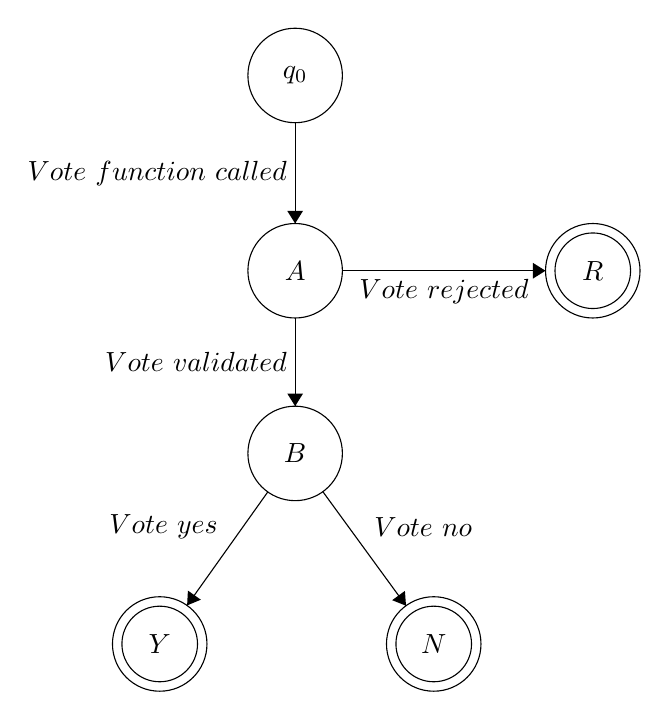
\begin{tikzpicture}[scale=0.2]
\tikzstyle{every node}+=[inner sep=0pt]
\draw [black] (36.9,-9.6) circle (3);
\draw (36.9,-9.6) node {$q_0$};
\draw [black] (36.9,-22) circle (3);
\draw (36.9,-22) node {$A$};
\draw [black] (36.9,-33.6) circle (3);
\draw (36.9,-33.6) node {$B$};
\draw [black] (55.8,-22) circle (3);
\draw (55.8,-22) node {$R$};
\draw [black] (55.8,-22) circle (2.4);
\draw [black] (45.7,-45.7) circle (3);
\draw (45.7,-45.7) node {$N$};
\draw [black] (45.7,-45.7) circle (2.4);
\draw [black] (28.3,-45.7) circle (3);
\draw (28.3,-45.7) node {$Y$};
\draw [black] (28.3,-45.7) circle (2.4);
\draw [black] (36.9,-12.6) -- (36.9,-19);
\fill [black] (36.9,-19) -- (37.4,-18.2) -- (36.4,-18.2);
\draw (36.4,-15.8) node [left] {$Vote\mbox{ }function\mbox{ }called$};
\draw [black] (36.9,-25) -- (36.9,-30.6);
\fill [black] (36.9,-30.6) -- (37.4,-29.8) -- (36.4,-29.8);
\draw (36.4,-27.8) node [left] {$Vote\mbox{ }validated$};
\draw [black] (39.9,-22) -- (52.8,-22);
\fill [black] (52.8,-22) -- (52,-21.5) -- (52,-22.5);
\draw (46.35,-22.5) node [below] {$Vote\mbox{ }rejected$};
\draw [black] (38.66,-36.03) -- (43.94,-43.27);
\fill [black] (43.94,-43.27) -- (43.87,-42.33) -- (43.06,-42.92);
\draw (41.89,-38.27) node [right] {$Vote\mbox{ }no$};
\draw [black] (35.16,-36.05) -- (30.04,-43.25);
\fill [black] (30.04,-43.25) -- (30.91,-42.89) -- (30.09,-42.31);
\draw (32.01,-38.28) node [left] {$Vote\mbox{ }yes$};
\end{tikzpicture}
\end{center}

This formal model provides the foundation for our conception of DAO smart contracts. As our goal is to verify the voting functionality of DAOs, it follows that we are focused primarily on the \textit{Vote Validated} event transition, and this is where most of our verification efforts will take place. Defining what it means for a vote to be validated will lead us to introduce our security properties.

\subsection{Security Properties for Secure DAO Voting}

\section{Approach}
Our approach uses Scribble and Mythril together to formally verify critical correctness properties in Ethereum-based DAO voting contracts. To begin, we identify essential governance rules found in most DAO implementations and articulate them into specific safety and liveness properties. Some key requirements include only token holders being able to vote, as well as prevention of double counting votes. These rules are expressed through Scribble annotations, which convert informal governance assumptions into precise assertions that are embedded into the Solidity contract. 

Our verification approach targets three core properties critical to DAO smart contract security. First, we verify Single Vote Enforcement, confirming that each member is restricted to casting only one vote per proposal, preventing potential manipulation through multiple votes. Second, we ensure Authorized Access, validating that voting and proposal functionalities are limited exclusively to authorized DAO members, thus safeguarding against unauthorized interference. Lastly, we confirm Integrity of Proposal Outcome, ensuring the correctness and immutability of voting results once finalized, to protect decision-making from fraudulent or erroneous alterations. We annotate each property explicitly using Scribble, enabling Mythril to systematically verify these essential conditions.

Once the properties are specified, we recompile the smart contract code using Scribble, then analyze it using Mythril’s symbolic execution engine. Mythril traverses possible execution paths, trying to invalidate the assertions that were defined earlier. If any violation is discovered by Mythril, it returns a counterexample and a symbolic execution path that led to the issue.

Upon encountering counterexamples, we analyze whether these findings represent genuine logic flaws or overly restrictive specifications. If there is a genuine logic flaw, we will flag it for review, while the latter will cause us to refine our annotations. We will evaluate the performance of our verification framework by testing it on both authentic DAO contracts and synthetic contracts that are injected with known vulnerabilities. Our goal is to produce a streamlined workflow that runs lightweight yet rigorous annotation-driven formal verification to ensure that Ethereum-based DAO governance contracts are secure.

We will first test synthetically vulnerable smart contracts specifically designed to contain known security flaws related to DAO voting. This initial step allows us to validate the correctness of our verification techniques in detecting deliberate vulnerabilities. After establishing confidence in our methodology, we will progress to analyzing a realistic and manageable contract such as MolochDAO v2[14], to test our verification framework in a practical but simplified real-world scenario.

We began by successfully setting up Mythril and integrating Scribble annotations for formal verification. To validate our setup, we created a simplified DAO smart contract example, incorporating core DAO functionalities. We annotated the critical sections using Scribble to define security properties explicitly. Running Mythril against this annotated DAO allowed us to verify that our environment and workflow operate correctly, establishing a solid foundation for further verification of more complex real-world DAOs.



\section{Evaluation}

This project investigates whether symbolic execution can be used to verify the safety and liveness properties of DAO voting functions. It also explores the scalability of this approach when applied to more complex voting mechanisms and assesses whether the method can be adapted to different DAOs' smart contracts. If automation isn't feasible, we want to investigate the manual effort required for adaptation. Our experiments will involve both toy examples and open-source smart contracts, focusing on analyzing DAO voting logic and defining the properties needed to verify it.

\section{Plan of Work}
We have already begun by studying the relevant tools, Scribble and Mythril, in order to understand the specification language and the way Mythril verifies security properties after they have been defined by Scribble. Next, we wrote a simple DAO contract, defined a security property in Slither, and verified the property using Mythril as an end-to-end test of our research procedure. We will go on to define security properties for each voting vulnerability in each smart contract that we plan to test. Over the next week we will verify the first three DAO contracts in our suite, and then in the final week we will verify the last two along with our final write-up. Our expected goal is to verify three different security properties in these five contracts. Our stretch goal would be to verify these properties in 10 contracts, but at minimum we expect to fully verify these properties in three contracts from our test suite.

\section{Who Did What}
\begin{itemize}
    \item Aidan: Contributed to the Introduction, Threat Model, and References
    \item Anish: Contributed to the Approach, Set up repository, dependencies, and starter DAO contract/annotations
    \item Jeffrey: Contributed to the Background, State of the Art, and Evaluation sections
\end{itemize}

\begin{thebibliography}{00}
\bibitem{b1} J. Feist, G. Grieco, and A. Groce, “Slither: A static analysis framework for smart contracts,” 2019, pp. 8–15. doi: https://doi.org/10.1109/WETSEB.2019.00008. Available: \url{https://ieeexplore.ieee.org/abstract/document/8823898?casa_token=SNthQs5W2d0AAAAA:XwX332JMCkj3hw8XZd9nKBxe2bKJZ3v3yUNJ3jPtangZ3L2nISxh_rbY8fBW2zXkaWa0QnqgqVE}
\bibitem{b2} Z. Nehaï, P.-Y. Piriou, and F. Daumas, “Model-checking of smart contracts,” 2018, pp. 980–987. Available: \url{https://ieeexplore.ieee.org/abstract/document/8726806}
\bibitem{b3} J. He, M. Balunović, N. Ambroladze, P. Tsankov, and M. Vechev, “Learning to Fuzz from Symbolic Execution with Application to Smart Contracts,” Proceedings of the 2019 ACM SIGSAC Conference on Computer and Communications Security, pp. 531–548, Nov. 2019, Available: \url{https://dl.acm.org/doi/abs/10.1145/3319535.3363230?casa_token=5cBcZneJt7oAAAAA:sPluGu-gtO_db3qLqHUcylo4ksy4Rx0FBkiEBFom7You4VltkgLyZanIwgg-WHfLDVmrwmU0MbdpGA}
\bibitem{b4} N. Sharma and S. Sharma, “A Survey of Mythril, A Smart Contract Security Analysis Tool for EVM Bytecode,” Indian Journal of Natural Sciences, vol. 12, no. 75, Dec. 2022, Available:
\url{https://www.researchgate.net/profile/Swati-Sharma-171/publication/366391033_A_Survey_of_Mythril_A_Smart_Contract_Security_Analysis_Tool_for_EVM_Bytecode/links/639ecbdc095a6a77743c8073/A-Survey-of-Mythril-A-Smart-Contract-Security-Analysis-Tool-for-EVM-Bytecode.pdf}
\bibitem{b5} ConsenSysDiligence, “GitHub - ConsenSysDiligence/scribble: Scribble instrumentation tool,” GitHub, Apr. 09, 2025. Available:  
\url{ConsenSysDiligence, “GitHub - ConsenSysDiligence/scribble: Scribble instrumentation tool,” GitHub, Apr. 09, 2025. https://github.com/ConsenSysDiligence/scribble/tree/develop (accessed Apr. 10, 2025).}
\bibitem{6} S. Nakamoto, “Bitcoin: a Peer-to-Peer Electronic Cash System,” bitcoin.org, Oct. 2008. Available: 
\url{https://bitcoin.org/bitcoin.pdf}
\bibitem{7} V. Buterin, “Ethereum Whitepaper,” Ethereum, 2014. Available: 
\url{https://ethereum.org/en/whitepaper/}
\bibitem{8} P. Wackerow, “Introduction to smart contracts,” ethereum.org, Sep. 02, 2022. Available: 
\url{https://ethereum.org/en/developers/docs/smart-contracts/}
\bibitem{9} N. Szabo, “Smart Contracts,” www.fon.hum.uva.nl, 1994. 
\url{https://www.fon.hum.uva.nl/rob/Courses/InformationInSpeech/CDROM/Literature/LOTwinterschool2006/szabo.best.vwh.net/smart.contracts.html}
\bibitem{10} C. Jentzsch, “DECENTRALIZED AUTONOMOUS ORGANIZATION TO AUTOMATE GOVERNANCE,” 2016. Available: 
\url{https://lawofthelevel.lexblogplatformthree.com/wp-content/uploads/sites/187/2017/07/WhitePaper-1.pdf}
\bibitem{11} C. Shier et al., “Understanding a Revolutionary and Flawed Grand Experiment in Blockchain: The DAO Attack,” SSRN Electronic Journal, 2017, doi: 
\url{https://doi.org/10.2139/ssrn.3014782.}
\bibitem{12} “List of 41 DAOs (2025),” Alchemy, 2025. Available:
\url{https://www.alchemy.com/dapps/top/daos}
\bibitem{13} K. Nekrasov, “DAO Voting Vulnerabilities,” Mixbytes.io, 2024.
\url{https://mixbytes.io/blog/dao-voting-vulnerabilities}
\bibitem{14} HausDAO, “GitHub - HausDAO/Molochv2.1: Moloch DAO v2 with multi-summoner capabilities, plus register function for metadata.,” GitHub, 2020. Available:
\url{https://github.com/HausDAO/Molochv2.1}
\end{thebibliography}
\end{document}
